\documentclass[PianoDiQualifica.tex]{subfiles}
\begin{document}
		
\chapter{Ciclo di Deming o PDCA}
Ogni processo deve essere organizzato basandosi sul principio del miglioramento continuo (o \citGloss{ciclo di Deming}):
\begin{description}
	\item [Plan (pianificare)]: viene definito un piano che basandosi sulla definizione di problemi e obiettivi pianifica compiti, assegna responsabilità, studia il caso, analizza le cause della criticità e definisce azioni correttive; 
	\item [Do (eseguire)]: vengono implementate le attività secondo le linee definite durante la fase Plan;
	\item [Check (valutare)]: viene verificato l'esito delle azioni di miglioramento rispetto alle attese;
	\item [Act (agire)]: vengono applicate le correzioni necessarie per colmare le carenze rilevate e vengono standardizzate le attività correttamente eseguite.
\end{description}

\begin{figure}[htbp]
	\begin{center}
		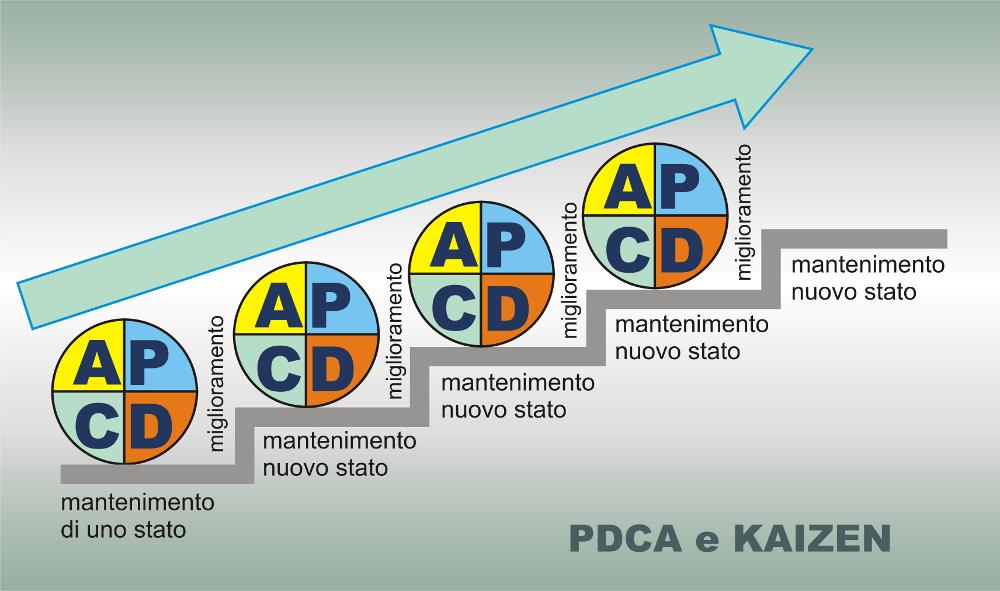
\includegraphics[width=0.7\linewidth]{PDCAkaizen}
		\caption[Ciclo di Deming]{Ciclo di Deming}
		\label{fig:pdca}
	\end{center}
\end{figure}

\end{document}